% !TEX program = pdflatex

\PassOptionsToPackage{unicode,breaklinks=true}{hyperref}
\documentclass[pdflatex,sn-mathphys]{sn-jnl}
\usepackage{graphicx}
\usepackage{booktabs}
\usepackage{multirow}
\usepackage{array}
\usepackage{float}
\usepackage{placeins}
\usepackage{xurl}


\makeatletter
\def\resultrows#1{\@@input #1 }
\let\headerps@out\@empty
\makeatother


\raggedbottom
\setlength{\textfloatsep}{8pt plus 2pt minus 2pt}
\setlength{\floatsep}{8pt plus 2pt minus 2pt}
\setlength{\intextsep}{8pt plus 2pt minus 2pt}
\setlength{\abovecaptionskip}{4pt}
\setlength{\belowcaptionskip}{2pt}
\renewcommand{\arraystretch}{1.08}

\graphicspath{{figures/}}

% =============================================================================
% =============================================================================




\makeatletter
\def\ps@headings{%
  \def\@oddfoot{\hfill}%
  \let\@evenfoot\@oddfoot%
  \def\@evenhead{\headerfont\thepage\qquad\rightmark\hfill}%
  \def\@oddhead{\headerfont\hfill\leftmark\qquad\thepage}%
  \let\@mkboth\markboth%
}%
\def\ps@titlepage{%
  \let\@oddhead\@empty\let\@evenhead\@empty%
  \def\@oddfoot{\vbox to 18pt{\vfill\reset@font\rmfamily\hfil\thepage\hfil}}%
  \def\@evenfoot{}%
}%
\makeatother

% ============================================================================
\jyear{2026}
\title[Choosing a Ranking for Low-Budget 4DGS]{Choosing a Primitive Ranking for Low-Budget 4D Gaussian Splatting}
\author[1]{\fnm{Guangzi} \sur{Zhang}}
\author[1]{\fnm{Yulong} \sur{Pan}}
\author[1]{\fnm{Conglin} \sur{Ma}}
\author[1]{\fnm{Kaijie} \sur{Qu}}
\author*[1]{\fnm{Xingquan} \sur{Cai}}
\email{caixingquan@ncut.edu.cn}
\affil[1]{\orgdiv{Beijing Key Laboratory of Cross-Modal Intelligent Immersive Computing}, \orgname{North China University of Technology}, \orgaddress{\city{Beijing}, \postcode{100144}, \country{China}}}
\abstract{A dynamic Gaussian scene can be rendered at a lower point count by ranking its primitives once and retaining a prefix. We ask how the choice of ranking depends on the source model, the target budget and subsequent optimization. We compare unrestricted analytical deletion influence with the same score applied only to the more opaque half of a trained source. At 10\% and 15\% retention, filtering improved test PSNR on all eight prefix-supervised sources in a paired scene comparison. On the eight ordinary seed-zero sources, unrestricted ranking led at both budgets. On Broom, Chicken and Flame Steak, a second independently trained ordinary source reproduced this direction. The 10\% Flame Steak advantage varied from 0.001 to 0.770~dB across seeds. These source families also differed in training configuration and model size. In a three-seed study, the filtering advantage on Chicken, Cut and Sear reversed at higher budgets and usually reversed after fixed-budget fine-tuning. On Cut, four scoring passes improved on one unrestricted pass at both budgets. A 30\% one-pass candidate pool attained higher mean quality at 10\%, while four passes led at 15\%.}

\keywords{4D Gaussian Splatting; dynamic novel-view synthesis; primitive selection; low-budget rendering}

\begin{document}
\maketitle

\section{Introduction}\label{sec:intro}
Dynamic Gaussian splatting represents a scene with explicit primitives whose rendered attributes change with time. A renderer can use a subset of an existing checkpoint to meet a primitive-count budget. At small budgets, the ordering matters because many splats compete to represent the same visible structure. A strongly opaque primitive may have little effect if an underlying splat has similar color, while a less opaque primitive may contribute distinctive detail across multiple views. We ask how much image quality a different ordering can recover at the same count.

We compare two ways to use the same single-removal influence score on an already trained dynamic scene. Unrestricted ranking (U) can retain any primitive. Candidate-restricted ranking (C) draws its smallest prefixes from the more opaque half. Within a source, these orders share the scoring observations, renderer, test frames and retained count. This design measures the effect of changing which points survive.

The clearest distinction emerged when we applied the two rules to different trained representations of the same eight scenes. At both low budgets, the direction of the C--U difference reversed between the available prefix-supervised and ordinary sources. Within the prefix-supervised family, we tested whether this ordering persisted as the budget grew and after equal fine-tuning. We also compared one-pass filtering with recomputing scores as the compositing context changes. Separate capacity controls, native renderer measurements and package sizes address what those quality differences cost in practice.

\section{Related Work}
\paragraph{Dynamic Gaussian rendering.}
3D Gaussian Splatting models appearance with anisotropic primitives that are depth ordered and alpha composited~\cite{kerbl20233d}. Dynamic Gaussian models use persistent primitives, deform canonical Gaussians, or model space and time directly~\cite{luiten2024dynamic,wu20244d,yang2024deformable,li2024spacetime,duan20244d}. We use the canonical Gaussian and time-conditioned deformation formulation of Wu et al.~\cite{wu20244d}, which uses plane-factorized features related to HexPlane~\cite{cao2023hexplane}. Scores computed from rendered observations can reflect changes in projected coverage and occlusion over time.

\paragraph{Nested budgets and pruning.}
Matryoshka Gaussian Splatting (MGS)~\cite{guo2026matryoshka} trains a static model with stochastic prefix and full-set supervision and uses descending opacity to construct nested prefixes. We apply opacity ranking to both ordinary 4DGS checkpoints and checkpoints trained with a local adaptation of this prefix-supervision principle. Each comparison of selection rules uses one frozen source. Pruning and compression studies also consider primitive importance and representation size~\cite{fan2024lightgaussian,niedermayr2024compressed,navaneet2024compgs}. The single-removal color perturbation follows the alpha-compositing identity underlying GaussianPOP~\cite{lee2026gaussianpop}, which applies analytical error estimates to static Gaussian simplification and also studies iterative rescoring. We aggregate this perturbation over time-conditioned observations and examine a fixed ranking with and without an opacity filter.

\section{Method}\label{sec:method}
\subsection{Checkpoint and budget}\label{sec:checkpoint}
Let a trained 4DGS checkpoint contain $N$ canonical primitives with fixed IDs. Given a camera and time, the deformation field and renderer produce projected splats and pixel colors. A budget fraction $\rho$ specifies $K=\operatorname{round}(\rho N)$ retained primitives. An offline order supplies the first $K$ IDs for a given budget. The renderer separately orders contributing splats by depth for alpha compositing.

The prefix-supervised sources use a local adaptation of MGS to dynamic 4DGS. Every training update includes an opacity-ranked prefix and a full render, with equal weights on their $L_1$ losses. Native density control uses the full render. For each update a seeded stream draws an integer $t$ uniformly from $\{1,\ldots,999\}$ and indexes the zero-based, float32 grid \texttt{linspace(1,0,1000)}. The nominal training fraction is thus $1-t/999$, including zero. The training code rounds the fraction times the current point count and clamps the result to at least one primitive. Ordinary sources use standard 4DGS training with prefix supervision disabled. We set the evaluation fraction independently. Within each checkpoint, ranking comparisons hold weights, test observations and $K$ fixed. Across independently trained sources, the full point count can differ.

\subsection{Analytical removal influence}
For calibration observation $v$, consider the depth-sorted tile candidates on a ray through pixel $x$ that pass the scorer's alpha threshold. The scorer caps effective alpha at $0.99$, drops contributions below $1/255$, and traverses the whole candidate sequence without the display renderer's transmittance cutoff. Let $\alpha_{vxi}$ denote the effective screen-space alpha of splat $i$, $\mathbf{c}_{vxi}$ its RGB color, and $T_{vxi}$ the product of $(1-\alpha)$ over the preceding accepted splats. Let $\mathbf{B}_{vxi}$ be the color composited from the accepted splats behind $i$ and the scene background, with incoming transmittance one. Up to a foreground term shared by both renders, the color with $i$ included is $T_{vxi}[\alpha_{vxi}\mathbf{c}_{vxi}+(1-\alpha_{vxi})\mathbf{B}_{vxi}]$. Omitting $i$ from that fixed ray sequence yields $T_{vxi}\mathbf{B}_{vxi}$. The difference gives the mean squared RGB score
\begin{equation}
S_i=\frac{1}{\lvert\mathcal V\rvert}\sum_{v\in\mathcal V}\frac{1}{3H_vW_v}
\sum_{x:\,i\ {\rm accepted}}
(T_{vxi}\alpha_{vxi})^2
\left\lVert\mathbf{c}_{vxi}-\mathbf{B}_{vxi}\right\rVert_2^2.
\label{eq:deletion-score}
\end{equation}
The scoring kernel replays the full source's accepted ray contributors with a backward suffix color recurrence initialized from the scene background. We use all pixels in 32 training observations per source in the primary comparison. Each observation specifies a camera and timestamp. Calibration uses the source render without target RGB values, and scores are averaged across views after division by each image's pixel and channel count.

Every score uses the full source as compositing context, including when the pool of eligible candidates is restricted. Pruning changes the context for the remaining splats and can change where the display renderer terminates a ray. The score estimates single-removal effects under the scoring kernel's compositing model and serves as a proxy for jointly pruning many splats. It supplies neither joint subset optimization nor a guarantee of monotonic PSNR.

\subsection{Nested orders and fixed-budget adaptation}
Let $o$ be the permutation by descending activated canonical opacity and let $K_b=\operatorname{round}(bN)$. We evaluate four orders using the same $N$ and $K$ within each source and budget.
\begin{itemize}
\item \textbf{O (opacity).} Use $o$ directly.
\item \textbf{C (candidate-restricted influence).} Rerank the first $K_{0.5}$ entries of $o$ using Eq.~\eqref{eq:deletion-score} and append the rest in opacity order.
\item \textbf{U (unrestricted influence).} Rank all $N$ primitives using Eq.~\eqref{eq:deletion-score}. Rendering uses exactly $K$.
\item \textbf{P (protected prefix).} Preserve the first $K_{0.1}$ entries of $o$, rerank the next entries up to $K_{0.5}$ by influence, and append the remaining entries in opacity order.
\end{itemize}
Score ties are resolved by ascending canonical ID. O and P have identical membership at 10\% by construction. C and P share the opacity candidate set at 50\%, with distinct smaller prefixes. C and U form the primary contrast. Their difference at the same $K$ measures the effect of restricting eligibility before influence ranking. O provides the opacity truncation baseline, and P isolates the effect of protecting an opacity prefix. We keep the 50\% definition of C fixed across source families and evaluate other widths separately on Cut.

The four orders produce subsets directly from the source for evaluation without adaptation. A separate experiment applies the same optimization protocol to each 15\% subset for 2,000 steps. Membership remains fixed, and the resulting checkpoints are specific to the 15\% budget. The original checkpoints and orders support selection at other budgets.

\section{Experiments}
\label{sec:experiments}

\subsection{Evaluation protocol}
\label{sec:setup}
The source-family comparison pairs ordinary and prefix-supervised checkpoints across eight scenes (Table~\ref{tab:sourcefilter}). We additionally test independent ordinary training runs on three scenes (Table~\ref{tab:ordrep}). For budget sweeps and matched adaptation, we use three prefix-supervised checkpoints per scene on four scenes: Chicken (HyperNeRF VRIG~\cite{park2021hypernerf}, 164 frames at $268\times480$), Cut Roasted Beef and Sear Steak (DyNeRF/N3DV~\cite{li2022neuralvideo}, 300 frames each at $480\times360$), and Basin (NeRF-DS~\cite{yan2023nerf}, 668 frames at $240\times135$). These scenes and test views had been examined previously. The independent runs quantify variation across training seeds within a scene.

For each source and nominal retained fraction, O, P, C and U have identical integer capacity $K$ and use identical test cameras. For the four-scene study we average raw PSNR over frames within each checkpoint, then report the scene mean and sample standard deviation over the three checkpoint values. Paired differences compare methods within each checkpoint before aggregation. All quality cells contain PSNR. Each auxiliary metric (SSIM and LPIPS) is missing for 46 archived Basin cells: ten at 10\% retention and twelve each at 15, 20 and 35\%. We leave these entries missing. The source-family comparison, within-scene repeats and supplemental 13-scene P/O study are reported separately.

\subsection{Ranking choice across source representations}\label{sec:sourcefamily}
We tested whether the benefit of restricting candidates changes with the source representation. We held the scene, camera sequence and retained fraction fixed, and compared C with U within each source. We used ordinary 4DGS checkpoints whose saved training configurations disabled prefix supervision. In addition to Chicken, Cut and Sear, we included all five additional real scenes with both an ordinary seed-zero checkpoint and a prefix-supervised source in the prepared-scene archive. These scenes had previously been examined under a different selection protocol. All low-budget comparisons used the same 50\% candidate pool and the same 32 training observations within scene. The comparison addresses transfer between existing sources. Training configurations and final point counts also differ between source families.
\begin{table}[!htbp]\centering\small
\caption{Effect of restricting the influence ranking to the more opaque half of the source. Entries give cold C minus U in mean test PSNR (dB). Both families use seed zero. Each difference compares equal point counts and identical frames within a trained source.}\label{tab:sourcefilter}
\begin{tabular}{lrrrr}\toprule
&\multicolumn{2}{c}{Prefix-supervised}&\multicolumn{2}{c}{Ordinary 4DGS}\\
Scene & 10\% & 15\% & 10\% & 15\% \\\midrule
Chicken & +0.528 & +0.074 & -1.742 & -2.830 \\
Cut Roasted Beef & +1.144 & +0.462 & -0.356 & -0.270 \\
Sear Steak & +0.923 & +0.386 & -0.191 & -0.101 \\
Coffee Martini & +1.092 & +0.521 & -0.356 & -0.720 \\
Flame Steak & +0.618 & +0.290 & -0.001 & -0.187 \\
Broom & +0.577 & +0.179 & -5.820 & -6.973 \\
3Dprinter & +0.120 & +0.032 & -1.966 & -2.937 \\
Peel Banana & +0.387 & +0.080 & -0.683 & -0.982 \\
\bottomrule\end{tabular}\end{table}
Across the eight paired seed-zero scenes in Table~\ref{tab:sourcefilter}, C exceeded U on every prefix-supervised source at both budgets. On ordinary Broom, restricting the candidate pool reduced PSNR by 5.820 and 6.973~dB at 10\% and 15\%, respectively. Appendix~\ref{sec:absolute} gives the native full counts and absolute full, O, C and U PSNR for every pair. U led on all eight ordinary sources at both budgets, with a near tie on Flame Steak at 10\%. On the ordinary Cut source at 10\%, U and C still exceeded opacity by 10.309 and 9.952~dB, respectively. The influence score remains useful on this source even though the filter reduces its benefit.


\runinheading{3}{Independent ordinary training runs.}
We repeated the comparison on three scenes selected from Table~\ref{tab:sourcefilter} to span different seed-zero gaps at 10\%: Broom (largest), Chicken (intermediate) and Flame Steak (smallest). These are within-scene training repeats. We evaluated an existing second Broom checkpoint and trained Chicken and Flame Steak from initialization with a second seed. Each run used the original ordinary scene configuration, 3,000 coarse and 30,000 fine updates, with prefix supervision disabled. The seed pairs shared prepared data, 32 training-only calibration observations, held-out frames and budget rules. Each checkpoint was evaluated at its own native count and at both fixed fractions. Table~\ref{tab:ordrep} gives individual paired effects; the public archive gives absolute full/O/C/U values and individual frame measurements.

\begin{table}[!htbp]\centering\small
\caption{Ordinary 4DGS training repeats. Each cell is U minus C in mean held-out frame PSNR (dB) for one independently trained checkpoint. Both orders retain exactly the same number of primitives within a cell.}\label{tab:ordrep}
\begin{tabular}{lrrrr}\toprule
 & \multicolumn{2}{c}{10\% retention} & \multicolumn{2}{c}{15\% retention}\\
Scene & Seed 0 & Seed 1 & Seed 0 & Seed 1 \\\midrule
Broom & +5.820 & +4.211 & +6.973 & +4.923 \\
Chicken & +1.742 & +2.097 & +2.830 & +3.351 \\
Flame Steak & +0.001 & +0.770 & +0.187 & +1.072 \\
\bottomrule\end{tabular}\end{table}
For the second ordinary Broom, Chicken and Flame Steak sources, U minus C was +4.211, +2.097 and +0.770~dB at 10\% retention, respectively. At 15\%, the corresponding differences were +4.923, +3.351 and +1.072~dB.

Figure~\ref{fig:broom10} shows where the loss occurs on a held-out frame. C breaks up the continuous pavement around the broom and introduces high-contrast streaks across the ground. U recovers the pavement boundary and broom silhouette, although the bristles and fine pavement texture remain softer than the reference. The whole-frame PSNR is 12.74~dB for C, 19.06~dB for U and 23.11~dB for the full source.
\begin{figure}[!htbp]\centering
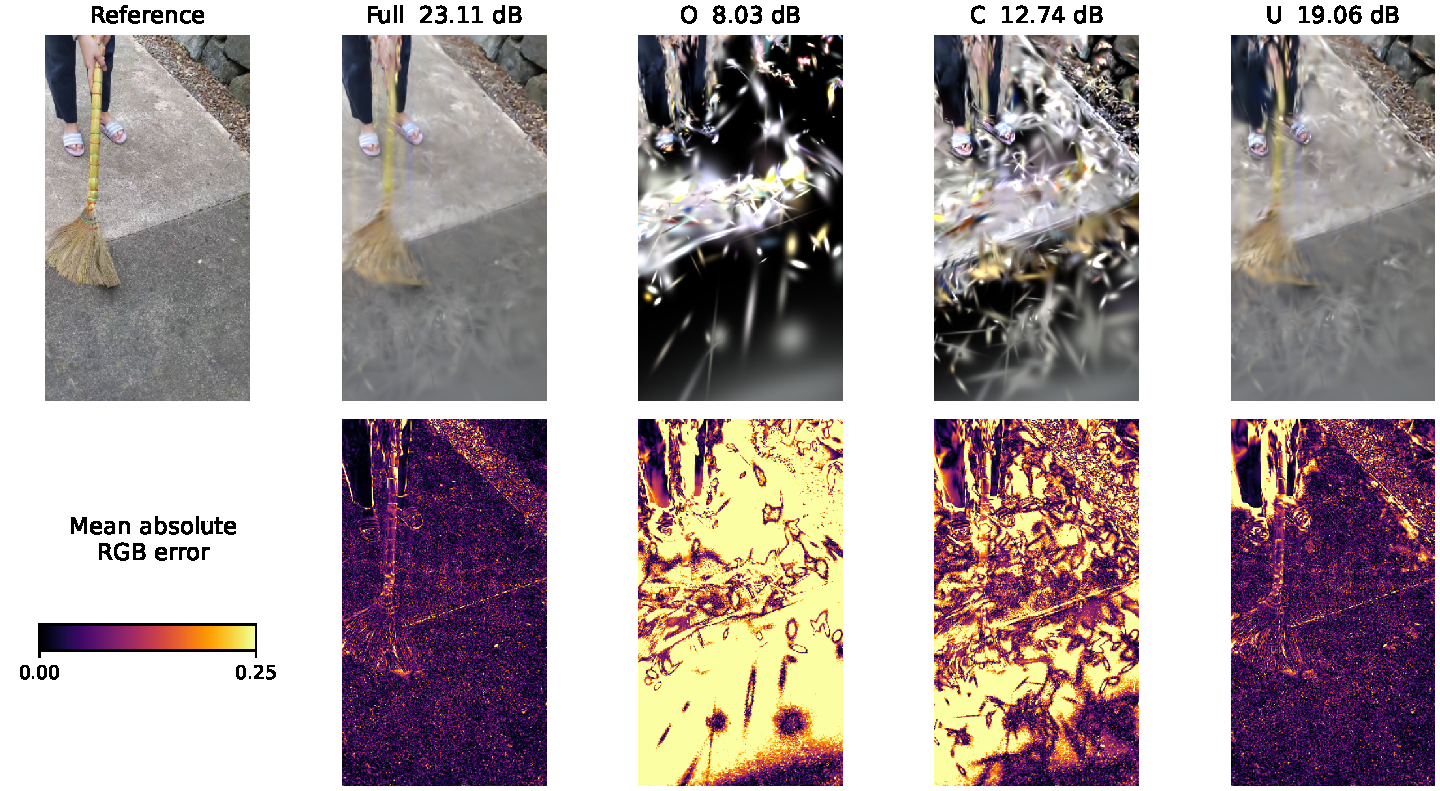
\includegraphics[width=\linewidth]{broom_10.pdf}
\caption{Ordinary Broom at 10\% retention (seed zero, 7,886 of 78,863 points). From left to right: reference image, full source, opacity (O), restricted influence (C) and unrestricted influence (U). Each label is whole-frame PSNR against the reference. The lower row shows mean absolute RGB error on the same linear scale, clipped at 0.25 on $[0,1]$ images. We chose the middle of the 197 held-out frames by list position (zero-based index 98), independently of frame quality.}\label{fig:broom10}\end{figure}


\subsection{Budget dependence before fine-tuning}
\label{sec:cold}
Table~\ref{tab:cold} and Fig.~\ref{fig:budget} report the same 240 quality cells across five budgets. At 10\%, C improves on opacity ranking (O) by 5.14~dB on Chicken, 2.26~dB on Cut and 1.55~dB on Sear, with improvements above 1~dB for every checkpoint from those three scenes. The respective differences at 15\% are 2.35, 1.85 and 1.06~dB, and at 20\% they narrow to 1.35, 1.45 and 0.76~dB. Basin has a smaller response throughout, with 0.11 and 0.09~dB gains at 10 and 15\%. The absolute values show that the small Basin gain occurs around 19.5~dB in this evaluation.

Comparing C with U isolates the opacity candidate restriction for the same analytic score. At both 10 and 15\%, C scores higher for all nine checkpoints from Chicken, Cut and Sear. At 20\%, C is ahead for two of nine checkpoints, and at 25 and 35\%, U is ahead for all nine. Basin differences between these variants are negligible. P and O select the same members at 10\% because P protects the opacity core at that budget. Additional 25\% controls hold the protected core and candidate band fixed (Table~\ref{tab:scorebridge}).

\begin{table*}[t]
\centering\small
\caption{Cold PSNR (dB), mean $\pm$ sample standard deviation across the three source checkpoints per scene. All four arms share the same sources, test frames and retained count for each budget.}
\label{tab:cold}
\resizebox{\linewidth}{!}{%
\begin{tabular}{lrcccc}
\hline
Scene & Budget (\%) & O & P & C & U \\
\hline
\resultrows{results_assets/cold.tex}
\hline
\end{tabular}}
\end{table*}

\begin{figure*}[t]
\centering
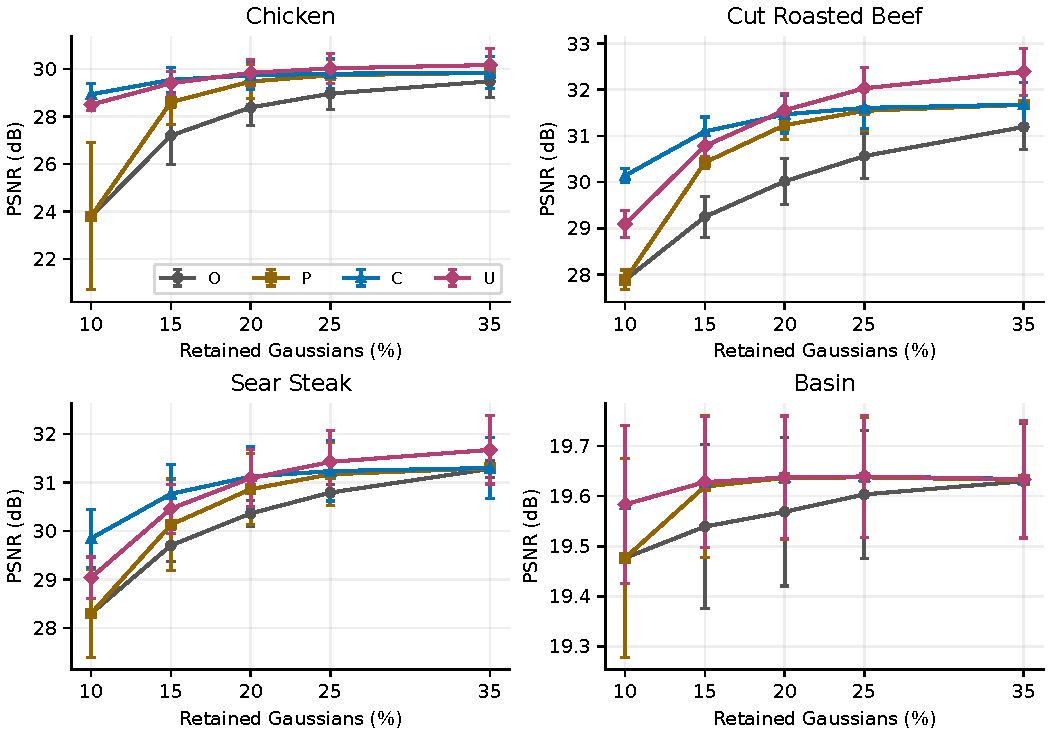
\includegraphics[width=.86\textwidth]{results_assets/budget.pdf}
\caption{Cold PSNR by retained fraction using the measurements in Table~\ref{tab:cold}. Error bars show one sample standard deviation across three checkpoints. The vertical scale varies by scene.}
\label{fig:budget}
\end{figure*}

\subsection{Ranking choice after matched fine-tuning at 15\%}
\label{sec:finetune}
For every source and ranking, we materialize the selected members at 15\% and apply 2,000 optimizer updates using common optimizer settings and the same training-camera schedule. Each run uses Adam to minimize $0.8L_1+0.2(1-\mathrm{SSIM})$ on training images, updating the retained point parameters and trainable deformation parameters. The endpoint is fixed in advance and test PSNR plays no part in choosing it. The membership remains fixed, with densification and member replacement disabled. The step-zero evaluations reproduce the archived cold per-frame PSNR with a maximum absolute deviation of $7.11\times10^{-15}$~dB. Table~\ref{tab:finetune} reports the fixed step-2,000 endpoint. Opacity subsets also benefit from the matched adaptation. The C--O gap remains positive for every Chicken, Cut and Sear checkpoint and exceeds 1~dB in all six Chicken and Cut pairs. U--O is negative for one Sear checkpoint ($-0.03$~dB), despite a positive scene mean. After fine-tuning, U exceeds C for eight of the nine Chicken, Cut and Sear checkpoints. P is below C for all nine. In Table~\ref{tab:finetune}, paired U minus C averages $+0.171$~dB on Chicken and $+0.566$~dB on Cut. On Sear the mean is $+0.002$~dB; its paired sample standard deviation, $0.452$~dB, reflects opposing changes across seeds. On Basin the mean difference is below 0.001~dB. Each adapted checkpoint serves its own 15\% working point.

\begin{table*}[t]
\centering\small
\caption{Matched fine-tuning at 15\%, PSNR (dB). Each entry is a mean $\pm$ sample standard deviation over three source checkpoints. The last column summarizes within-checkpoint differences.}
\label{tab:finetune}
\resizebox{\linewidth}{!}{%
\begin{tabular}{lccccc}
\hline
Scene & O & P & C & U & U--C \\
\hline
\resultrows{results_assets/finetune.tex}
\hline
\end{tabular}}
\end{table*}

\subsection{Candidate-pool width and repeated scoring}\label{sec:reschedule}
We then tested how much one-pass ranking loses when the compositing context changes. On each of the three prefix-supervised Cut sources, the unrestricted four-pass comparator rescored the survivors after retaining 60\%, 35\%, and 20\% of the full set. The final scoring pass supplied both target counts. This adapts the iterative re-quantification principle of GaussianPOP to a shared fixed-count schedule. No optimizer updates were applied. The same camera--time observations were used on every pass.
\begin{table}[!htbp]\centering\small
\caption{Cut Roasted Beef, three prefix-supervised sources. Mean $\pm$ sample SD over three sources for PSNR and offline preparation time on the RTX 3090. Time includes scoring, ordering and intermediate subset formation after warm-up, with model and cameras resident. Peak PyTorch allocation averaged 578.4~MiB for each scored variant. Single-pass pool variants share the full-source scoring measurement.}\label{tab:rescore}
\begin{tabular}{lrrr}\toprule
Selection & 10\% (dB) & 15\% (dB) & Prep. (s) \\\midrule
Opacity & $27.882\pm0.216$ & $29.250\pm0.440$ & --- \\
One pass, 30\% pool & $30.332\pm0.378$ & $30.816\pm0.489$ & $0.544\pm0.002$ \\
One pass, 50\% pool & $30.141\pm0.152$ & $31.097\pm0.313$ & $0.593\pm0.037$ \\
One pass, 70\% pool & $29.277\pm0.244$ & $30.868\pm0.246$ & $0.552\pm0.003$ \\
One pass, all candidates & $29.093\pm0.286$ & $30.782\pm0.268$ & $0.554\pm0.003$ \\
Four passes, all candidates & $30.185\pm0.361$ & $31.385\pm0.374$ & $1.478\pm0.098$ \\
\bottomrule\end{tabular}\end{table}
Relative to unrestricted one-pass scoring, four passes recovered 1.092 and 0.602~dB at 10\% and 15\%, respectively. At 10\%, the 30\% one-pass pool exceeded four passes by $0.147\pm0.215$~dB (paired mean and sample SD, two of three seeds). For the 50\% pool the corresponding difference was $-0.045\pm0.265$~dB. At 15\%, four passes exceeded the strongest one-pass pool (50\%) by $0.288\pm0.205$~dB and led on all three seeds. The 30\% and 50\% widths summarize the observed sweep on Cut. Selecting the width for a new scene would require a rule fixed independently of its test results.

With model and calibration cameras resident and kernels warmed, the original timing used one measurement per method and source. Each ordering supplied both target budgets in the same preparation, including the final pass of the four-pass schedule. Four passes averaged 1.478~s versus 0.593~s for one pass with the 50\% pool. The additional 0.885~s is paid once when the ordering is reused across frames. In a separate timing check we repeated each procedure five times per source, alternating order and materializing both endpoints in each timed run. Mean and sample SD across the 15 measurements were $0.504\pm0.037$~s for the 50 percent pool and $1.322\pm0.034$~s for four passes. Section~\ref{sec:runtime} reports frame latency.

\FloatBarrier
\subsection{Quality relative to the full source}
\label{sec:full}
For all four scenes, the archived 100\% renders use every Gaussian from the same source checkpoints used for subset selection. Chicken, Cut and Sear use direct native all-ID renders. Basin uses the archived full-count opacity render from the same evaluation as its cold 25\% subsets. Table~\ref{tab:full} reports the paired gap to those references. At 10\%, C is 1.31--2.37~dB below the full source on the Chicken, Cut and Sear scene means. The gap is 0.69--1.42~dB at 15\% and 0.44--0.90~dB at 25\%. Adapting the 15\% subset reduces the mean gap to 0.01--0.63~dB. Basin has a much smaller full-source gap across the reported working points. At 25\%, mean SSIM decreases by 0.017, 0.016 and 0.013 on Chicken, Cut and Sear, respectively, while mean LPIPS increases by 0.030, 0.015 and 0.010. To express the 15\% results as a working-point choice, we count sources whose mean PSNR is at most 0.5 or 1.0~dB below their full source. After matched adaptation, C meets these descriptive cutoffs on 9/12 and 12/12 sources, respectively, compared with 4/12 and 5/12 for O. The cold gaps measure the effect of subsetting the frozen source. The final column combines subsetting and additional optimization.

\begin{table*}[t]
\centering\small
\caption{Full-source PSNR and paired differences (full minus C, dB). Entries show mean $\pm$ sample standard deviation across the same three checkpoints per scene. The 100\% column uses the unpruned source checkpoint.}
\label{tab:full}
\resizebox{\linewidth}{!}{%
\begin{tabular}{lccccc}
\hline
& & \multicolumn{4}{c}{Full minus C} \\
Scene & Full (100\%) & Cold 10\% & Cold 15\% & Cold 25\% & Fine-tuned 15\% \\
\hline
\resultrows{results_assets/full.tex}
\hline
\end{tabular}}
\end{table*}

\subsection{Rendering latency and profiling}
\label{sec:runtime}
We measured synchronous native rendering on one RTX 3090 (PyTorch 2.5.1+cu121, CUDA 12.1), using resident test cameras at the quality-evaluation resolutions. The dynamic path gathers the selected indices from the full source at runtime and uses the deformation network and rasterizer. The compact path uses a materialized subset and runs deformation and rasterization. The measurements exclude model preparation, offline ranking, quality metrics, and file output. We pool frame timings over three traversals of the entire test split within one process for each working point and source. We compute p50 and p95 within that pool, form each method's ratio to O within source, and report the median across sources. These measurements describe resident native rendering. Section~\ref{sec:delivery} reports package sizes and a separate HTTP payload test.

Figure~\ref{fig:cost} shows quality and median frame latency at the five cold budgets. Table~\ref{tab:timing} reports the corresponding latency statistics for the fine-tuned compact subsets. Over the nine Chicken, Cut and Sear sources, the median paired C/O time ratio is 1.021 at p50 and 1.032 at p95, and U/O is 1.029 and 1.047. The C/O p95 ratio reaches 1.116 on Cut, so similar median times can coexist with a larger tail cost. Within a fixed count, methods may still produce different projected footprints and pixel overlap, which affect the rasterizer's workload.

The stage measurements in Table~\ref{tab:profile} use separate synchronization and 12 fixed test cameras for each instrumented working point. At cold dynamic 15\%, deformation medians of 2.36--3.22~ms exceed the gather (0.15--0.18~ms) and raster (0.53--0.78~ms) medians in the illustrated configurations. Those independently instrumented medians describe the size of each stage. Frame latency is measured separately. The persistent deformation cost helps explain why latency does not scale in proportion to the retained Gaussian count in these runs. Increasing cold C retention from 10\% to 25\% increased p50 frame time for all 12 sources on both paths. The median paired increase was 1.246~ms with dynamic gathering and 1.215~ms with a compact subset. On each path, p95 increased for 11 of 12 sources.

\begin{figure*}[t]
\centering
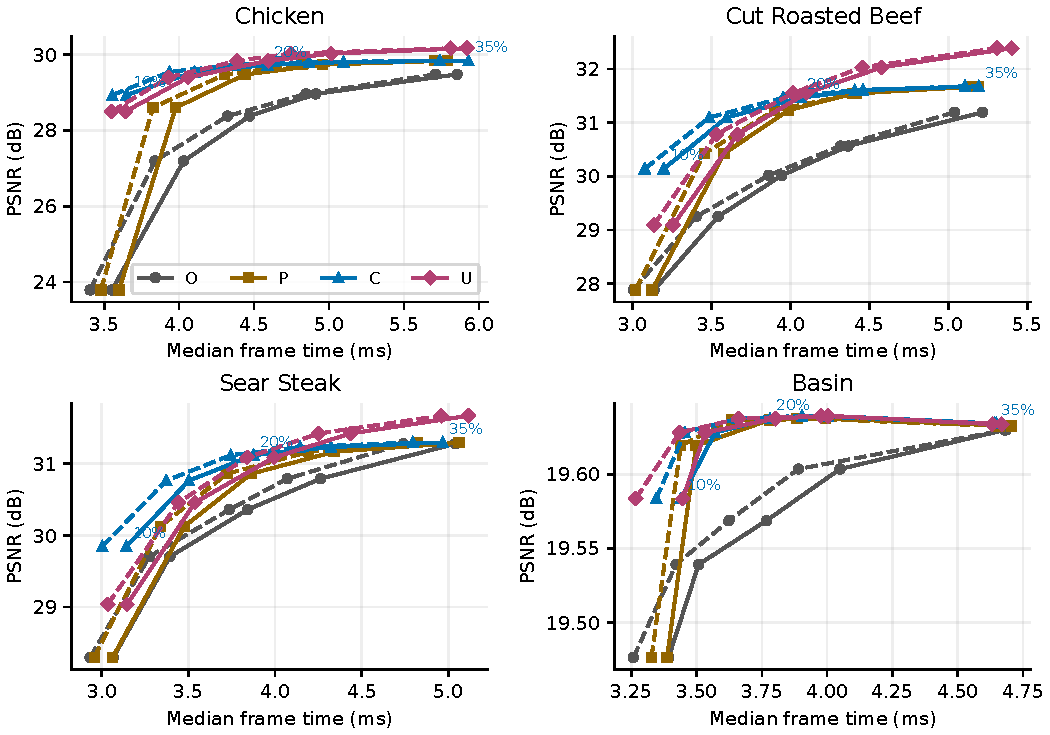
\includegraphics[width=.86\textwidth]{results_assets/cost.pdf}
\caption{Cold PSNR versus measured resident-render latency. Each point combines mean PSNR and the median of the three source-level p50 frame times for the same arm and retained count. Solid lines show dynamic gathering and dashed lines show compact subsets. Lines connect observations in budget order. Dynamic C is annotated at 10, 20, and 35\%.}
\label{fig:cost}
\end{figure*}

\begin{table*}[t]
\centering\small
\caption{Fine-tuned 15\% compact frame latency. Each entry is the median across three sources of the displayed statistic. The last two columns first form the corresponding latency ratio to O within each source.}
\label{tab:timing}
\begin{tabular}{lccccc}
\hline
Scene & Arm & p50 (ms) & p95 (ms) & p50/O & p95/O \\
\hline
\resultrows{results_assets/timing.tex}
\hline
\end{tabular}
\end{table*}

\begin{table*}[t]
\centering\small
\caption{Separately instrumented cold dynamic stages at 15\% for O, C, and U. Entries are medians across sources of stage medians in milliseconds.}
\label{tab:profile}
\begin{tabular}{lcccc}
\hline
Scene & Arm & Gather & Deformation & Rasterization \\
\hline
\resultrows{results_assets/profile.tex}
\hline
\end{tabular}
\end{table*}



\section{Discussion}\label{sec:discussion}
The choice between C and U depended first on the trained representation. At the same retained fractions, all eight scene pairs favored filtering on their prefix-supervised source and unrestricted ranking on their ordinary source. On ordinary Broom, excluding the lower-opacity half cost 5.820~dB at 10\% retention and 6.973~dB at 15\%. On ordinary Flame Steak, the 10\% U advantage varied from 0.001~dB at seed zero to 0.770~dB at seed one. At 10\%, the two ordinary Broom sources favored U by 5.820 and 4.211~dB, and the two Chicken sources by 1.742 and 2.097~dB. The repeat compares effect sizes within deliberately selected scenes; only one ordinary source is available for each of the other five scene pairs. A plausible explanation is that opacity rank aligns differently with the primitives needed for reconstruction in the two families. Density, redundancy and final point count could also contribute. Distinguishing these explanations would require changing one training factor at a time.

Within the prefix-supervised family, direct-rendering gains also depended on the retained count. Across all nine Chicken, Cut and Sear checkpoints, C exceeded U at both 10\% and 15\%, while U exceeded C at 25\% and 35\%. After matched adaptation at 15\%, U exceeded C in eight of the nine. The ranking that gives the better immediate rendering can therefore differ from the ranking that gives the better initialization for further optimization.

Filtering and rescoring change different decisions. Filtering changes which points are eligible, whereas rescoring updates the estimated effect of deletion after other points have gone. On Cut, four passes beat the best tested one-pass setting at 15\%, but the 30\% one-pass pool led on average at 10\%. For a reusable ordering, the original 0.885~s difference is an offline charge shared by both target budgets and subsequent frames. Its practical weight depends on how often the ordering is regenerated.

Absolute quality puts the ranking gains in perspective. On ordinary Chicken at 10\%, opacity truncation gives 9.830~dB, unrestricted influence gives 21.421~dB and the full source gives 31.097~dB. Changing the order recovers 11.591~dB at the same point count, while the full source retains a 9.676~dB advantage over U. On Basin, the 15\% subset approaches full-source quality and changing its order adds only about 0.09~dB over opacity. The first comparison quantifies the value of selection under a severe constraint. The second shows that a good low-budget image can also come from a source where ranking makes little difference.

\paragraph{Choosing a ranking for a new checkpoint.}
For direct rendering at 10--15\%, our paired results motivate trying U first on ordinary sources resembling those tested and C alongside U on prefix-supervised sources. A larger prefix or planned adaptation changes that choice: on Chicken, Cut and Sear, U led across the three prefix-supervised replicates at 25--35\% and in eight of nine comparisons after 15\% fine-tuning. For a new checkpoint, reserve validation cameras and timestamps before inspecting test quality. Compare O, C and U at the intended count, using the same validation frames and the intended adaptation schedule. If repeated scoring is affordable, include it with both its validation quality and its one-time preparation time. Freeze the choice before the final test. For near ties, inspect paired differences by validation camera and time interval before assigning a preference. For new training pipelines and untested budgets, these comparisons provide starting candidates; the validation comparison determines the choice.

\section{Conclusion}\label{sec:conclusion}
A fixed opacity filter changes the value of influence ranking differently across trained representations. The eight available prefix-supervised sources in the paired scene comparison benefited at both low budgets, while their ordinary 4DGS counterparts favored unrestricted influence. The direction persisted in second ordinary training runs on three scenes, with appreciable variation in magnitude. Larger retained sets and matched fine-tuning also favored U on most of the repeatedly tested strong-response sources. On Cut, filtering and iterative rescoring offered distinct quality and preparation-time trade-offs. These comparisons support evaluating a ranking at the intended source, point budget and optimization regime.

\section*{Acknowledgments}
This work was supported by the National Natural Science Foundation of China (No.~61503005), the Humanities and Social Sciences Fund of the Ministry of Education of China (No.~22YJAZH002), the Beijing Natural Science Foundation (No.~L253018), and the Beijing Education Science Planning Project (No.~CCDA25172), Digital Twin Teacher-Assisted Teaching Application Practice Research.

\section*{Statements and Declarations}
\textbf{Competing interests.} The authors declare that they have no conflict of interest.

\textbf{Data and code availability.} The experiments use public dynamic-scene datasets, including NeRF-DS~\cite{yan2023nerf}. The \href{https://github.com/leokingpan/random-budget-4dgs/tree/62f82c4c466db33753bb189b48d0cc9987ccccee/studies/source-ranking}{versioned study materials} include the scoring implementation, archived measurements, case inputs and verification commands. The CPU case reconstructs selected point IDs from archived scores and recomputes mean PSNR from stored frame measurements. Generating predictions and PSNR from pixels requires the corresponding trained checkpoint, prepared camera and image records, the deformation model loader and a compatible native CUDA rasterizer. The repeat data also identify each checked model and retained count.

\textbf{Author contributions.} G.Z. and Y.P. designed the study. Y.P. implemented the algorithms, conducted experiments, and analyzed the data. C.M. prepared figures and tables and contributed to dataset preparation, baseline experiments, and ablation validation. K.Q. contributed to baseline experiments and ablation validation. G.Z. and Y.P. wrote the manuscript. X.C. supervised the project and advised on experimental design and manuscript structure.

\textbf{Ethics approval.} Not applicable.

\textbf{Consent to participate.} Not applicable.

\clearpage\appendix
\section{Absolute reconstruction quality by source}\label{sec:absolute}
Each row reports seed zero, the same test frames within scene, and mean per-frame PSNR in dB. Full denotes native full-source rendering. O, C and U use the same number of points within each source and budget. The CSV accompanying the manuscript also gives the exact retained count.
\begin{table}[!htbp]\centering\footnotesize\caption{Prefix-supervised sources. Absolute PSNR at full capacity and at 10\% and 15\% retention.}\begin{tabular}{lrrrrrrrr}\toprule
& & &\multicolumn{3}{c}{10\%} &\multicolumn{3}{c}{15\%}\\ Scene & Full count & Full & O & C & U & O & C & U \\\midrule
Chicken & 176,950 & 30.344 & 21.897 & 29.141 & 28.612 & 26.491 & 29.707 & 29.633 \\
Cut Roasted Beef & 205,825 & 32.081 & 27.987 & 30.109 & 28.966 & 28.926 & 30.999 & 30.537 \\
Sear Steak & 192,453 & 32.195 & 28.526 & 30.287 & 29.364 & 29.656 & 31.220 & 30.834 \\
Coffee Martini & 285,974 & 27.052 & 24.828 & 25.598 & 24.505 & 25.716 & 26.309 & 25.788 \\
Flame Steak & 197,484 & 31.413 & 26.903 & 29.846 & 29.228 & 28.719 & 30.638 & 30.348 \\
Broom & 201,107 & 22.680 & 21.758 & 22.179 & 21.601 & 22.002 & 22.362 & 22.183 \\
3Dprinter & 361,999 & 22.517 & 19.364 & 22.427 & 22.307 & 21.001 & 22.473 & 22.442 \\
Peel Banana & 364,260 & 24.224 & 18.772 & 22.715 & 22.329 & 20.340 & 23.444 & 23.364 \\
\bottomrule\end{tabular}\end{table}
\begin{table}[!htbp]\centering\footnotesize\caption{Ordinary sources. Absolute PSNR at full capacity and at 10\% and 15\% retention.}\begin{tabular}{lrrrrrrrr}\toprule
& & &\multicolumn{3}{c}{10\%} &\multicolumn{3}{c}{15\%}\\ Scene & Full count & Full & O & C & U & O & C & U \\\midrule
Chicken & 110,454 & 31.097 & 9.830 & 19.679 & 21.421 & 10.961 & 22.081 & 24.911 \\
Cut Roasted Beef & 94,350 & 33.344 & 14.098 & 24.050 & 24.406 & 15.426 & 26.983 & 27.253 \\
Sear Steak & 83,772 & 33.298 & 11.970 & 24.074 & 24.265 & 17.093 & 26.880 & 26.981 \\
Coffee Martini & 128,573 & 28.742 & 11.856 & 19.135 & 19.491 & 12.260 & 21.567 & 22.287 \\
Flame Steak & 87,532 & 33.145 & 15.614 & 24.545 & 24.546 & 16.231 & 27.227 & 27.414 \\
Broom & 78,863 & 22.490 & 8.229 & 12.562 & 18.382 & 9.123 & 12.867 & 19.840 \\
3Dprinter & 187,479 & 22.822 & 12.019 & 17.903 & 19.869 & 14.479 & 18.560 & 21.498 \\
Peel Banana & 267,505 & 26.945 & 9.879 & 17.231 & 17.914 & 10.358 & 19.868 & 20.850 \\
\bottomrule\end{tabular}\end{table}

\clearpage\section{Supplementary protocols and controls}\label{sec:supp}
\subsection{Source-training variants}
For the earlier submitted training variant, each iteration added prefix supervision with probability 0.5, drawing the fraction uniformly from $[0.1,1]$ on that branch. Section~\ref{sec:method} specifies the discrete schedule for the prefix-supervised sources used in the ranking comparisons.
\subsection{Validation against physical single-point deletion}
We compared the predicted RGB mean squared error (MSE) with the change in the display renderer after physically removing one point. For Cut seed zero we used four training observations, stratified by score rank and supplemented with points where C and U disagreed. The matched analysis comprises 96 point--view pairs from 68 distinct canonical point IDs. Every ID in these pairs belongs to the 15\% U subset. Removing the same ID in the full source and in that subset therefore defines both measurements. Each context has 28 pairs with exactly zero measured perturbation. Repeated views of the same point are not independent replicates.

Over all 96 pairs, the pooled Spearman correlation was 0.9985 in the full source. In the reduced context, the full-source score gave 0.9609 and the score recomputed in the subset gave 0.9986. To assess magnitude, among the 68 pairs per context with measured MSE above $10^{-15}$, the median predicted-to-measured ratio was 1.000 in both contexts. The 10th--90th percentile intervals were 0.963--1.007 (full) and 0.959--1.016 (subset). Figure~\ref{fig:deletion_check} shows the individual errors. These comparisons validate single-point perturbations on the sampled views. The PSNR comparisons between complete pruning schedules measure the effect of removing many points together.
\begin{figure}[htbp]\centering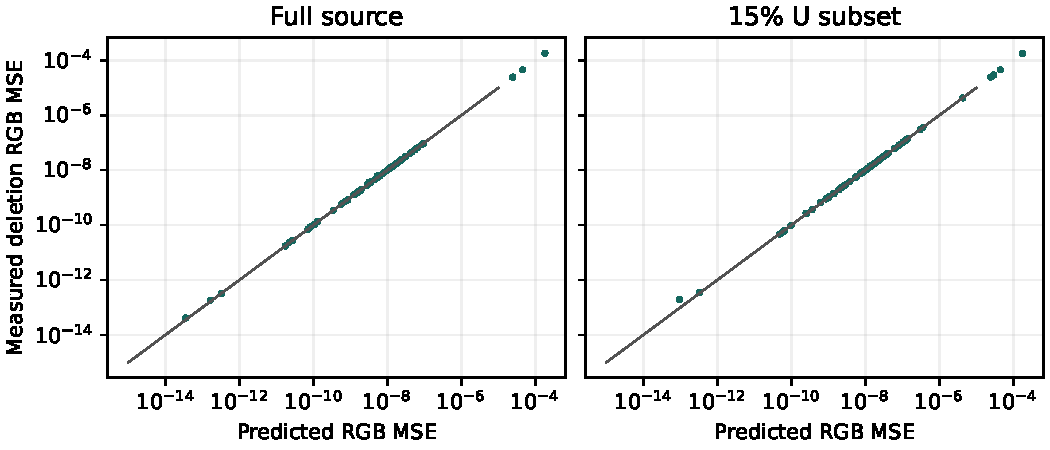
\includegraphics[width=.94\linewidth]{deletion_magnitude.pdf}
\caption{Predicted and measured MSE in each point's current rendering context. Only pairs with both values positive appear on logarithmic axes. The diagonal denotes equal predicted and measured errors.}\label{fig:deletion_check}\end{figure}
\subsection{Calibration coverage across time}
On the prepared scenes, the calibration procedure selects equally spaced ranks among the available training times and cycles among the cameras available at those times. On Cut seed zero, we varied the observation count (8, 16, 32 and 64) and the initial camera offset (0, 6 and 12). At 10\% retention, C yielded 29.765--29.944~dB using eight observations, 30.058--30.138~dB using 32, and 30.075--30.117~dB using 64. Figure~\ref{fig:time_cut} shows the framewise comparison for the original 32 observations.
\begin{figure}[htbp]\centering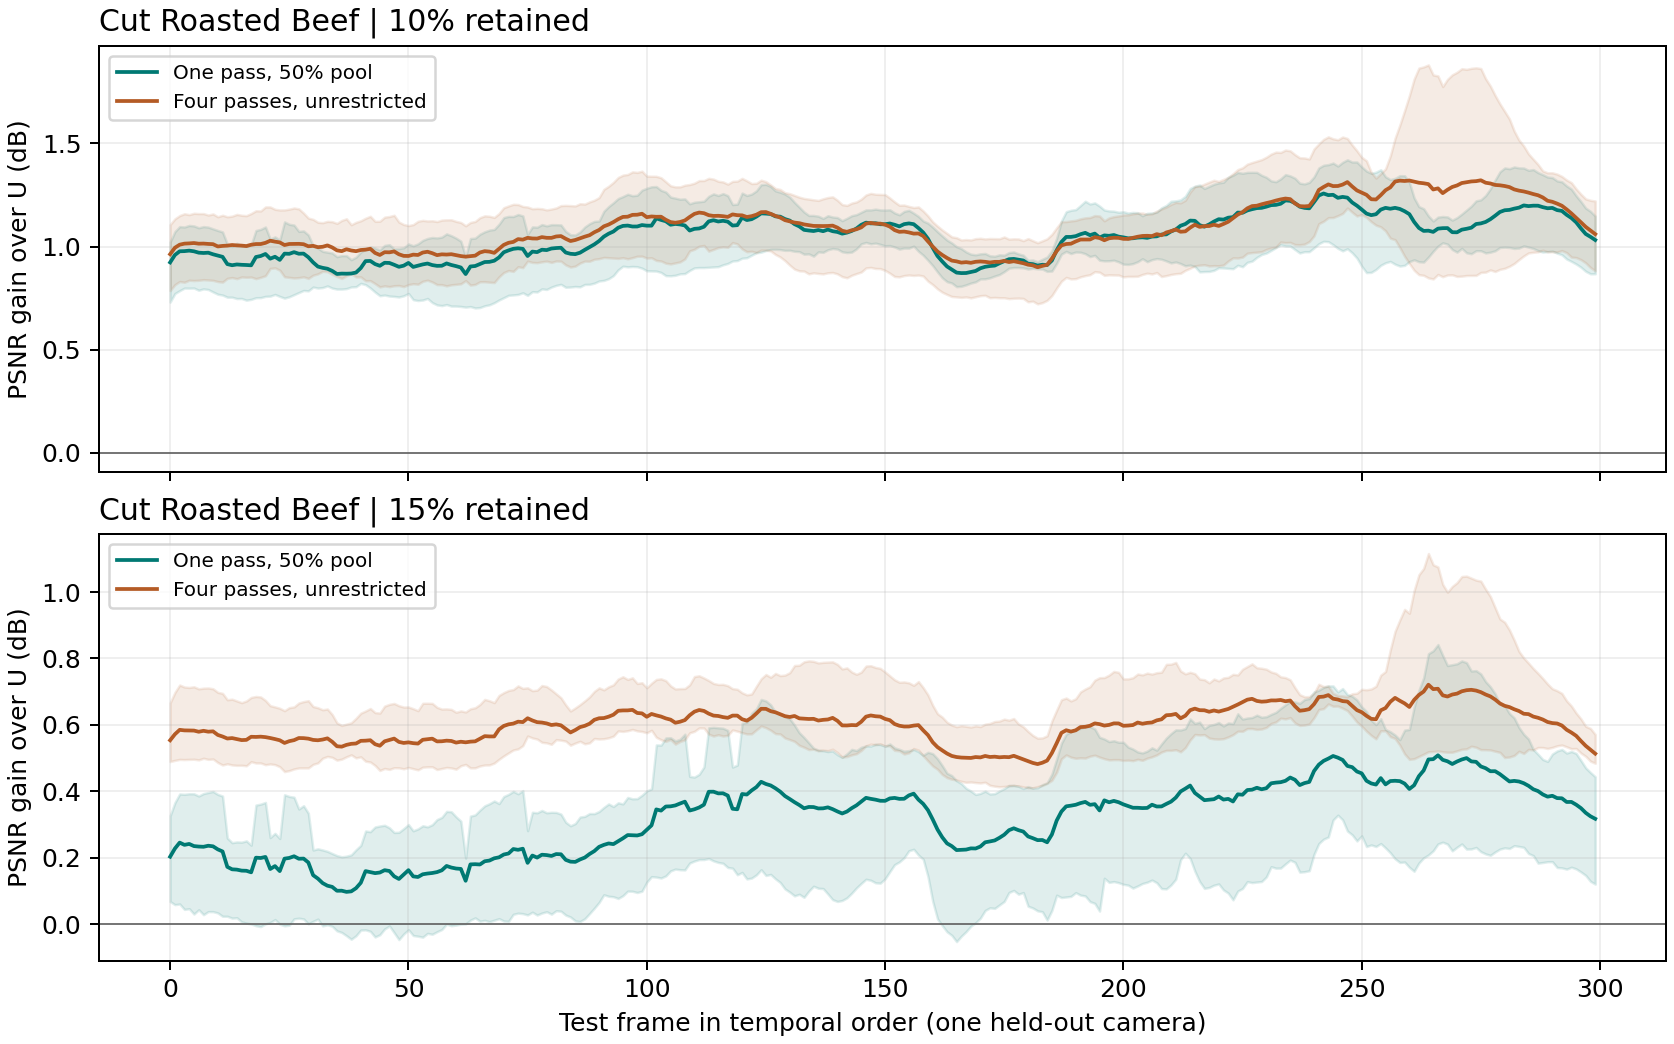
\includegraphics[width=\linewidth]{temporal.png}
\caption{Quality relative to one unrestricted pass, in the temporal order of the 300 held-out Cut frames. Lines show means across three prefix-supervised sources. Shading spans the three source values per frame.}\label{fig:time_cut}\end{figure}

\subsection{Comparing two rankings across 13 real scenes at 25\% retention}
\label{sec:historical}
Table~\ref{tab:historical} compares opacity and protected-core rankings at 25\% retention across 13 real scenes from three dataset families. Each row uses one source checkpoint and reports the endpoint after 2,000 fine-tuning steps on both opacity (O) and protected-core (P) subsets. P gains in 11 scenes, by at least 0.5~dB in five and at least 1~dB in one. Gains are small in the NeRF-DS scenes and two of those pairs favor O. Table~\ref{tab:sourcefilter} compares C and U across two source families in eight paired scenes. The budget and adaptation experiments use four prefix-supervised scenes with three sources each.

\begin{table*}[t]
\centering\small
\caption{Opacity and protected-core rankings at 25\% retention after 2,000 matched fine-tuning steps, with one source per scene. Absolute PSNR and paired differences are in dB.}
\label{tab:historical}
\begin{tabular}{llrrr}
\hline
Dataset & Scene & O & P & P--O \\
\hline
\resultrows{results_assets/historical.tex}
\hline
\end{tabular}
\end{table*}

\subsection{Independent fixed-capacity training}
\label{sec:capacity}
We also evaluate a model trained separately for each of two 25\% targets (Chicken and Cut, one source per scene). Each run trains for 33,000 updates with a Gaussian capacity constraint during densification and reaches its target exactly. O, P and C use cold subsets of the corresponding existing source at that identical count. The cold C subset exceeds the matched capacity model by 2.02~dB on Chicken and 0.15~dB on Cut. The independently trained model is 1.92~dB below P on Chicken and 0.10~dB below P on Cut. On Cut, independent training has better SSIM (0.931 versus 0.924 for P), while P has lower LPIPS (0.071 versus 0.089). The independent capacity runs took 910.4 and 938.7 seconds on Chicken and Cut, using full-only supervision plus native regularization. The corresponding reusable sources took 2,159 and 2,226 seconds with full and prefix supervision. Each trained source supplies all five cold budgets from the same weights.

\begin{table*}[t]
\centering\small
\caption{Independent 25\% fixed-capacity training control. Each comparison uses the same target count $K$ and matched test views. Training seconds refer to the separately trained capacity model's training loop. Quality is PSNR (dB).}
\label{tab:capacity}
\setlength{\tabcolsep}{3pt}\begin{tabular}{lrrrrrr}
\hline
Scene & $K$ & Fixed capacity & Cold O & Cold P & Cold C & Train (s) \\
\hline
\resultrows{results_assets/capacity.tex}
\hline
\end{tabular}
\end{table*}

\subsection{Comparison with opacity times scale area}
For comparison we also evaluate an earlier opacity--scale product. Its implementation uses
\begin{equation}
s_i^{\mathrm{legacy}}(t)
=\operatorname{sigmoid}(\widetilde o_i(t))\,
s_{ix}^{\mathrm{can}}s_{iy}^{\mathrm{can}},
\label{eq:legacy-score}
\end{equation}
where $\widetilde o_i(t)$ is the opacity logit returned by the deformation module and $s_{ix}^{\mathrm{can}}$ and $s_{iy}^{\mathrm{can}}$ are activated canonical scale components. Opacity deformation is disabled in the archived comparison configurations, so the product is time invariant there. The two scale components are in canonical coordinates. The main comparison uses the rendering-based score in Eq.~\eqref{eq:deletion-score}.


\subsection{Ranking within a fixed opacity band}\label{sec:bridge}
An earlier matched experiment held the opacity core, candidate band, source and count fixed and changed the ordering within the band. The comparators used the opacity--scale product in Eq.~\eqref{eq:legacy-score}, one frozen random order per source, or a feedback-based protected ordering (H). The first two controls isolate the contribution of the ranking within the same band. H also changes the calibration procedure.
\begin{table}[htbp]
\centering
\caption{Effect of changing the ranking within the protected band at 25\% retention. Each entry is the mean paired difference in cold PSNR (P minus comparator, dB) across three sources. Positive values favor P.}\label{tab:scorebridge}
\begin{tabular}{lrrr}
\toprule
Scene & Opacity--scale & Random order & Feedback (H) \\
\midrule
Chicken & +3.0496 & +2.6040 & -0.0418 \\
Cut roasted beef & +2.1925 & +2.4405 & -0.0331 \\
Sear steak & +2.1149 & +2.2713 & -0.0305 \\
Basin & +0.0133 & +0.0750 & +0.0003 \\
\bottomrule
\end{tabular}
\end{table}

P outperformed the opacity--scale product and the fixed random order on all twelve sources. Feedback yielded higher PSNR than P on eleven. The latter improvement adds an offline cost: on Chicken, Cut roasted beef and Sear steak, the median selection time over three independent processes was 3.22--3.37 times as long for H as for P. Including loading and saving reduced the ratio to 1.49--1.57. These measurements compare the preparation cost of P and H only. Peak allocated memory during selection was higher for P.\par

\subsection{What remains visible at one quarter of the points}\label{sec:visual}
Figure~\ref{fig:visual} compares the same test view across the observation, the complete source, and three cold subsets. In all three frames, reranking recovers part of the quality lost under opacity truncation. We also compared the central $192\times144$ pixels against ground truth for all nine archived example views (three per scene, seed 0). In the 8-bit images, full-source crop PSNR exceeded cold C crop PSNR in all nine pairs, by 0.047--0.757~dB. The crop measurements quantify local reconstruction error, whereas the labels in the figure describe the entire frame.
\begin{figure}[htbp]
\centering
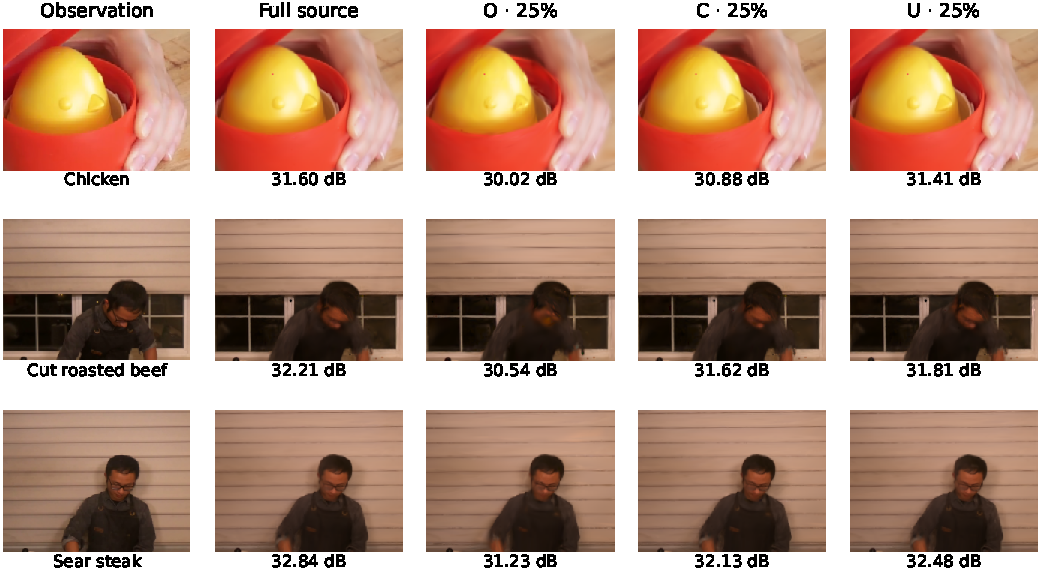
\includegraphics[width=\linewidth]{qualitative.pdf}
\caption{Matched central crops at 25\% retention. Each row uses seed 0 and the middle of three archived example views (source indices 165, 150, and 150, respectively). Each crop spans the central $192\times144$ native pixels. Values below the renderings give PSNR for the entire corresponding frame. The full-source column uses all points from the same source as the three subsets.}\label{fig:visual}
\end{figure}

For Press, a separate historical experiment on the protected-core order P contains 487 paired $240\times135$ test frames per seed across three seeds. At 25\% retention the mean full-minus-P PSNR gap is 0.018~dB, while the largest individual frame gap is 0.353~dB. These frame averages characterize the archived Press runs. The original figure used a separate rendering record.

\subsection{Model storage and transfer}\label{sec:delivery}
For each of the 12 sources, we serialized both the complete model and its cold C subset at 15\% retention. Both packages use an uncompressed archive of the native binary point cloud, deformation network, point-indexed deformation table, render settings and canonical point IDs. All 24 archives passed CPU round-trip checks. Removing points reduces the point-indexed payload while preserving the shared deformation network.
\begin{table}[htbp]
\centering\small
\caption{Payload size of complete and 15\% C models in decimal MB. Sizes are scene means over three checkpoints. Savings are the range of within-checkpoint reductions.}\label{tab:delivery}
\begin{tabular}{lrrr}\toprule
Scene & Full (MB) & C (MB) & Savings (\%) \\\midrule
Chicken & 78.15 & 37.08 & 51.3--53.3 \\
Cut Roasted Beef & 63.26 & 17.88 & 71.6--71.8 \\
Sear Steak & 59.97 & 17.39 & 70.7--71.4 \\
Basin & 76.16 & 48.41 & 36.4--36.5 \\\bottomrule
\end{tabular}
\end{table}
For Chicken seed 0 we served both packages over a loopback HTTP connection. The client received 75,314,041 bytes for the full model and 36,659,192 bytes for C, a 51.3\% reduction in response-body bytes. Both received files matched the source SHA-256 digests. This test measures the data to be delivered. Frame timings in Section~\ref{sec:runtime} were measured with the native RTX 3090 renderer.
At the same cold C 15\% membership and resident test cameras, rendering the materialized subset reduced peak PyTorch-allocated GPU memory by 29.0--47.0~MiB relative to gathering from the full model, across all 12 native RTX 3090 source pairs.

\subsection{Full-capacity comparison with independently trained standard 4DGS}\label{sec:basin_native}
For Basin, we compared standard 4DGS with the prefix-supervised source at each model's native full count. The three seed pairs shared the same initial point-cloud fingerprint within each pair. Each model received 17,000 training updates. We rendered the same 668 held-out frames at $240\times135$ on one RTX 3090, verified image and camera identities, and measured PSNR in a separate pass. For timing, we warmed up each model, synchronized each frame and alternated model order across three traversals and seeds. Both models rendered all of their primitives directly. Table~\ref{tab:basin_native} summarizes the paired evaluation.

\begin{table}[!htbp]\centering\small\caption{Basin full-capacity comparison. Entries are means over three seeds. Frame-time percentiles are computed within each model over 2,004 synchronized renders. Memory is peak PyTorch allocation. Recorded training-worker time includes startup checks and excludes queue time.}\label{tab:basin_native}\begin{tabular}{lrr}\toprule
Metric & Standard 4DGS & Prefix-supervised \\\midrule
Full primitive count & 93,267 & 127,031 \\
Test PSNR (dB) & 19.728 & 19.631 \\
Median frame time (ms) & 7.37 & 9.53 \\
95th-percentile frame time (ms) & 8.58 & 10.69 \\
Peak allocated memory (MiB) & 218.7 & 279.4 \\
Training-worker time (s) & 568.7 & 931.9 \\
\bottomrule\end{tabular}\end{table}

Standard 4DGS and the full prefix-supervised source attained 19.728 and 19.631~dB, respectively. The prefix-supervised source contained 36.2\% more points and its median frame time was 29.3\% higher. At 15\% of this source, cold C used approximately 19,055 points, or 20.4\% of the standard full-model count, and reached 19.63~dB (Table~\ref{tab:cold}). At this same subset count, C exceeded O by 0.09~dB. The first comparison quantifies the quality retained with fewer points. The second isolates the gain due to selection.


\FloatBarrier
\bibliography{references}
\end{document}
